\chapter{Introduction}

\section{Principles of Electron Cooling}
As a particle beam is traveling through a particle accelerator, the spread
of the particles must be kept to a minimum. All the particles should have
nearly the same momentum, low positional spread and as little transverse
velocity as possible. This minimizes the amount of particles that are lost
in the path to their destination, and maximizes the amount of collisions.

Electron coolers are used to decrease the transverse velocity for anti protons
or negative ion beams. The cooler is mounted along the beam path, as seen in
figure \ref{fig:ecooler}.

\begin{figure}[!h]
    \centering
    \includegraphics[width=0.8\textwidth]{figs/ecooler.png}
    \caption{An electron cooler.}
    \label{fig:ecooler}
\end{figure}

Electrons are shot from an electron gun into the gun solenoid. In the
first toroid section they are "kicked" into the beam path. Here, their
lateral speed is matched to that of the particle beam. The beam particles
will now collide with the electrons. Because both the beam particles and
the electrons are negatively charged, the transverse momentum will be
transferred to the electrons through Coulomb interactions. This in effect
reduces the latitudinal temperature of the beam. The now hot electrons are
then taken out of the beam path in the second toroid, into an electron collector.

The magnets in the cooler are weak, in the order of tens of milliteslas.
Because of this, they affect the path of the electrons by a large degree, but
not the path of the much heavier beam particles.

\begin{figure}
    \centering
    \begin{subfigure}[b]{0.4\linewidth}
        \centering
        \includegraphics[width=0.9\linewidth]{figs/epath}
        \caption{An electron moving forwards in a solenoidal magnetic field,
        with its velocity $v_e$ and Lorentz force $F_e$. Solenoidal field axis $B$ in red.}
        \label{fig:epath}
    \end{subfigure}
    \hfill
    \begin{subfigure}[b]{0.4\linewidth}
        \centering
        \includegraphics[width=0.9\linewidth]{figs/ecloud}
        \caption{A particle beam (red) and a
        surrounding electron cloud (blue).}
        \label{fig:ecloud}
    \end{subfigure}
    \caption{}
\end{figure}

Because the magnets in the cooler are solenoids, the electrons will follow a
spinning path through the cooler according to the Lorentz Force, as seen in 
figure \ref{fig:epath}. When a lot of electrons are shot through the cooler at
the same time, they produce a cylindrical electron cloud around the particle
beam, ensuring that any beam particles with to high of a temperature will
collide with the electron cloud. \cite{Tranquille2018-fs}
This is illustrated in figure \ref{fig:ecloud}. The functional operation
of the electron cooler is very dependent on the field quality in the 
main drift solenoid. Any non solenoidal field components will throw 
the electrons off their intended path, thus necessitating high quality
magnetic measurements of the cooler.

\section{Project Purpose and Goal}

\section{Previous Work}